\documentclass{article}

\usepackage[left=1.8in,right=1.8in,top=.6in,bottom=1in]{geometry}

\usepackage{assumptionsofphysics}
\usepackage{tikz}
\usetikzlibrary{positioning}
\usepackage{hyperref}
\hypersetup{
	colorlinks=true,
	citecolor=blue,
	urlcolor=blue,
	linkcolor=blue
}
\frenchspacing

\newcommand{\marginleft}[1] {\reversemarginpar\marginpar{#1}}
\newcommand{\marginright}[1] {\normalmarginpar\marginpar{#1}}

\def\ordinals{\textbf{ORD}}
\def\cardinals{\textbf{CRD}}

\def\ordless{\prec}
\def\ordleq{\preceq}
\def\ordeq{\sim}
\def\ordgeq{\succeq}

\def\crdleq{\hookrightarrow}
\def\crdeq{\leftrightarrow}
\def\crdgeq{\hookleftarrow}


\title{Bare minimum: SUBJECT}

\date{\vspace{-5ex}}
\begin{document}

\maketitle


\begin{abstract}
This note presents a condensed summary of SUBJECT which can function as a crash course, refresher and/or reference. Bare minima are meant to give a rough overview, by no means complete, of the subject to the intellectually curious, particularly in the context of foundational questions in physics.
\end{abstract}

\section{Introduction}

Brief overview

\emph{This work is part of Assumptions of Physics (\url{https://assumptionsofphysics.org}), a project that aims to identify a handful of physical principles from which the basic laws can be rigorously derived.}


\section{A topic}

Introductory comment of an informal nature.

\subsection{A subtopic}

\begin{defn}[Pop of a set - simple definition]
	The pop of a set $A$ \marginleft{Pop} is the curb of its power set.
\end{defn}

\begin{defn}[Foo sets - definition with properties]
	We say a set $A$ is \textbf{foo}
	\marginleft{Foo: $\circledcirc$}, noted $\circledcirc A$, if it satisfies the following properties:
	\begin{itemize}
		\item \textbf{Shirted}: the pop of $A$ is shirted
		\item \textbf{Intarred}: the pop of $A$ is a subset of the tar of $A$
	\end{itemize}
\end{defn}

\begin{defn}[Foo operations - multiple definitions]
	We define the following operations on foo sets:
	\begin{description}
		\item[Credit.] Noted $A \veebar B$, the credit of $A$ and $B$ is the smallest foo set that contains.
		\item[Change.] Noted $A \barwedge B$, the change of $A$ and $B$ is the biggest foo set that is contained by both.
	\end{description}
\end{defn}

\begin{remark}
	Highlight something important in the formal definitions or their use.
\end{remark}


\marginright{~\\
	\def\setA{ (-1,0) circle (2) }
	\def\setB{ (1,0) circle (2) }
	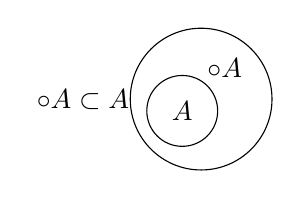
\begin{tikzpicture}[scale = 0.3]
		\draw (0.3,0) circle (3); 
		\draw (-0.5,-0.5) circle (1.5);
		\node at (-4.7,0) {$\circ A \subset A$};
		\node at (-0.5,-0.5) {$A$};
		\node at (1.3,1.3) {$\circ A$};
	\end{tikzpicture} 
}

\begin{defn}[Center - definition with a diagram]
	The \textbf{center} of a set $A$ \marginleft{Set center: $\circ A$}, noted $\circ A$, is the subset of all blorped elements.
\end{defn}


\bibliographystyle{plain}
\bibliography{bibliography}

\end{document}